\section{Data Geospasial}
Terdapat dua model data geospasial, yaitu model data raster dan model data vektor. 
Pada gambar \ref{datageospasial} dijelaskan tentang Klasifikasi model data geospasial.
\begin{figure}[ht]
	\centerline{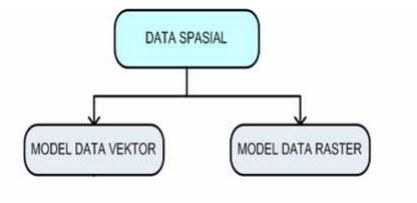
\includegraphics[width=1\textwidth]{figures/datageospasial.JPG}}
	\caption{Klasifikasi Model Data Geospasial.}
	\label{datageospasial}
	\end{figure}

\subsection{Data Vektor}
Model data vektor merupakan model data yang paling banyak digunakan dan dikenal pula sebagai model data spaghetti. Lembaran kertas peta ditranslasikan garis demi garis ke dalam list koordinat (x,y) dalam format digital. Sebuah titik dikodekan sebagai pasangan koordinat (x,y) tunggal. Sebuah garis dikodekan sebagai list atau string pasangan koordinat (x,y). Sementara area atau luasan dikodekan sebagai polygon.
Model ini berbasiskan pada titik dengan nilai koordinat (x,y) untuk membangun objek spasialnya. Objek yang dibangun terbagi menjadi tiga bagian lagi yaitu berupa titik (point), garis (line), dan area (polygon).

\subsubsection{Polygon}
Dalam artikel Mahendra menjelaskan Polygon merupakan representasi objek dalam dua dimensi. Contoh : danau,
persil tanah, dan lain-lain. Entity polygon dapat direpresentasikan dengan berbagai cara di dalam model data vektor. 
Struktur data polygon bertujuan untuk mendeskripsikan properties yang bersifat topologi dari suatu area sedemikian rupa sehingga properties yang dimiliki oleh blok-blok bangunan spasial dasar dapat ditampilkan dan dimanipulasi sebagai data peta tematik. Seperti halnya titik dan garis, area juga dapat menggambarkan objek yang berbeda menurut skalanya. Area dapat menggambarkan wilayah hutan atau sawah pada peta skala besar. 
Cara yang paling sederhana untuk merepresentasikan suatu poligon adalah pengembangan dari cara yang digunakan untuk merepresentasikan arc yang sederhana yaitu merepresentasikan setiap poligon sebagai sekumpulan koordinat (x,y) yang membentuk segmen garis, dimana mempunyai titik awal dan titik akhir segmen garis yang sama (memiliki nilai koordinat yang sama). Bentuk-bentuk dasar representasi data spasial ini, di dalam sistem model data vektor, didefinisikan oleh sistem koordinat kartesian dua dimensi (x,y). Di dalam model data spasial vektor, garis-garis atau kurva merupakan sekumpulan titik-titik terurut yang dihubungkan. Sedangkan luasan atau poligon juga disimpan sebagai sekumpulan list titik-titik, tetapi dengan catatan bahwa titik awal dan titik akhir poligon memiliki nilai koordinat yang sama dengan syarat poligon tersebur tertutup. Representasi vektor suatu objek merupakan suatu usaha di dalam menyajikan objek yang bersangkutan sesempurna mungkin. Untuk itu, ruang atau dimensi koordinat diasumsikan bersifat kontinyu yang memungkinkan semua posisi, panjang dan dimensi didefinisikan dengan presisi.
Fitur poligon adalah area tertutup seperti bendungan, pulau, batas negara dan sebagainya. Seperti fitur polyline, poligon diciptakan dari rangkaian simpul yang terhubung dengan garis kontinyu. Namun karena poligon selalu menggambarkan area tertutup, simpul pertama dan terakhir harus selalu berada di tempat yang sama! Poligon sering memiliki batas geometri bersama yang sama dengan poligon tetangga. Banyak aplikasi GIS memiliki kemampuan untuk memastikan bahwa batas-batas poligon tetangga persis sama. Kita akan membahasnya di topik Topology nanti di tutorial ini. Seperti halnya titik dan polyline, poligon memiliki atribut. Atribut menggambarkan masing-masing poligon. Misalnya bendungan mungkin memiliki atribut untuk kedalaman dan kualitas air.\cite{mahendra2014sistem}.


\subsubsection{Karakteristik Polygon}
- Titik distrukturisasi dan disimpan (direcord) sebagai satu pasang koordinat(x,y).
- Garis distrukturisasi dan disimpan sebagai suatu susunan pasangan koordinat(x,y) yang beraturan.
- Luasan distrukturisasi dan disimpan sebagai satuan susunan pasangan koordinat(x,y) yang berurutan yang menyatakan segmen-segmen garis yang menutup menjadi suatu poligon.

\subsubsection{Kelebihan}

1. Struktur datanya lebih rumit
2. Efisiensi untuk analisis
3. Sebagai sarana representasi yang baik
4. Transformasi proyeksi lebih efisien
5. Ketelitian, akurat dan lebih presisi
6. Relasi atribut langsung dengan DBMS (database)

\subsubsection{Kekurangan}

1. Sulit dalam melakukan proses overlay
2. Tidak bisa menampilkan data image/foto udara
4. Struktur data yang terlalu banyak tidak efektif dalam menampilkan banyak spasial
5. Memerlukan algoritma dan proses yang sangat kompleks
6. Kualitas (output) sangat bergantung dengan printer dan kartografi
7. Sulit dilakukan simulasi 
